\chapter{Paper 2 - Quantum Graph Neural Networks for Molecular Property Prediction}

\section*{Abstract}

Efforts to mitigate climate change are increasingly in the public eye. This includes hydrogen research and the study of molecular properties such as the potential energy surface, which provides information about the interaction of different materials. The potential of quantum computing to process information at the molecular or atomic level could enable fundamental advances in hydrogen research and computational chemistry. Therefore, this paper investigates the integration of graph neural networks (GNNs) with quantum computing to predict such molecular properties. To this end, fundamental work on quantum graph neural networks (QGNNs) is reviewed and key requirements for the development of such a model are identified. Despite the challenges of fully implementing a QGNN, a prototype Quantum Convolutional Neural Network (QCNN) is developed as a first step, and initial simulations show promising results. The research contributes to the understanding of quantum-enhanced machine learning models for molecular property prediction. These results provide a promising direction for future advances in computational chemistry, as well as materials science and the prediction of molecular proprties in the course of climate change mitigation. \\

\textit{\textbf{Keywords:} quantum computing, 
quantum machine learning, quantum graph neural networks, hydrogen research, potential energy surface prediction}

\section{Introduction}
\label{sec:introduction}

In view of the steadily advancing climate change, efforts to reduce environmental pollution are
increasingly coming into focus both in the public eye and within the scientific community \cite{amin_hydrogen_2022}.
This includes the search for scalable and cost-effective renewable energy storage solutions, which
is essential to meet the world's growing energy demand while mitigating climate change \cite{kilkis_research_2019}. The
conversion of electricity to hydrogen, as well as the reverse combustion process, can play an
important role here \cite{amin_hydrogen_2022}. Therefore, new materials are constantly being investigated to enable
catalytic processes in the field of hydrogen production to run efficiently \cite{chen_waste-derived_2023}. Machine learning
methods are already being used to simulate and calculate catalytic properties. In particular, graph
neural networks (GNN) are proving to be especially promising here \cite{tran_open_2023, bronstein2017geometric}. Since the prediction of potential energy surfaces and other relevant properties takes place at the molecular and atomic level, the use of quantum computing or quantum machine learning is an interesting direction of research in the field of molecular properties. There is currently a growing interest in exploring the application of quantum computers in various domains \cite{valdez2023review}. The results of Tychola et al., which are also shown in Figure \ref{img:tychola}, show that the number of publications in the field of quantum machine learning has drastically increased since 2017 and that German research is also making a significant contribution to this \cite{Tychola_Kalampokas_Papakostas_2023}.

\begin{figure}[h!]
    \begin{subfigure}{.5\textwidth}
     \captionsetup{justification=centering}
      \centering
      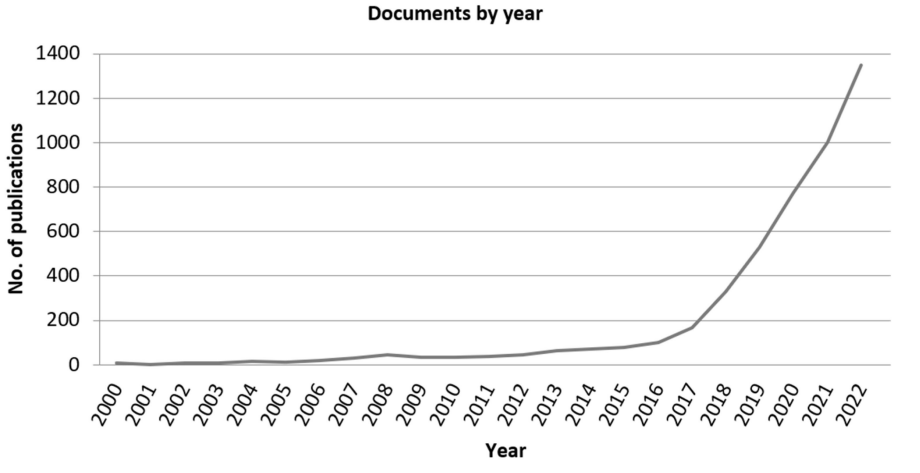
\includegraphics[width=.8\linewidth]{QML-Documents.png}
      \caption{Number of documents released per year in the field of QML}
      \label{fig:sfig1}
    \end{subfigure}%
    \begin{subfigure}{.5\textwidth}
      \centering
      \captionsetup{justification=centering}
      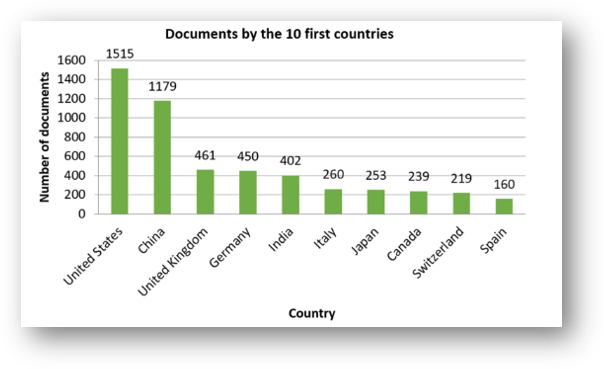
\includegraphics[width=.8\linewidth]{QML-countries..png}
      \caption{Number of documents released per country in the field of QML}
      \label{fig:sfig2}
    \end{subfigure}
    \caption[Results of QML-Literature-Overview from Tychola et al. 2023 (excerpt)]{\label{img:tychola} Results of QML-Literature-Overview from Tychola et al. 2023 \cite{Tychola_Kalampokas_Papakostas_2023} (excerpt)}
    \end{figure}

The literature also shows that first approaches to realize GNNs on quantum computers already exist \cite{verdon_quantum_2019, beer_quantum_2021,ai_decompositional_2023,zheng2021quantum,ryu2023quantum}. The resulting combination of quantum machine learning and graph neural network models is called Quantum Graph Neural Networks (QGNNs). However, the specific application of predicting molecular properties by using QGNNs, particularly in hydrogen research, remains underexplored in the literature. This provides an opportunity to bridge the gap between quantum computing and molecular science in the context of hydrogen storage and catalysis. \\
    
In order to solve the presented problem, the following research question and sub-questions are created: 

\begin{center}
    \textit{"How can a Quantum Graph Neural Network for the prediction of molecular properties be developed?"} \\
\end{center}
Q1: \textit{How do Quantum Graph Neural Networks work?} \\
Q2: \textit{How must molecular data be processed to be used with a quantum computer?} \\
Q2: \textit{How does the performance compare to classical Graph Neural Networks?} \\

The goal of this paper is to develop an understanding of QGNNs and how they work. Besides, in the scope of this paper, an understanding of the prediction of potential energy surfaces of molecules is created. Based on this procedure, the analysis of different foundation papers will show how a QGNN can be developed. In summary, to answer the developed research question and sub-questions, the following artifacts will be created as part of the research: 

\begin{itemize}
    \item foundation paper analysis of different papers in the context of quantum graph neural networks
    \item based on the foundation paper analysis: requirements analysis to identify the requirements for the development of a quantum graph neural network that is able to predict molecular properties 
    \item attempt to develop a quantum graph neural network based on the conducted requirement analysis
\end{itemize}  

The structure of this paper is as followed: first, the scientific foundations and theoretical background are discussed. Then the research methodology is presented in detail. Based on this, the findings and their results are presented and then discussed. Finally, a conclusion and discussion of the results is provided, as well as an overview of possible research topics based on this work.   

\section{Theoretical Background}
\subsection{Quantum Computing}
In order to understand the fundamentals of quantum computing, it is first necessary to explain the basic building blocks of quantum computing. These are also known as quantum bits, quantum gates and quantum circuits, and are explained in the following. In quantum computing, quantum bits, or qubits, are the basic units of information. Unlike classical bits, which can only take the states 0 or 1, qubits operate according to the principles of quantum mechanics, which allows them to take both states simultaneously. \cite{claudino2022basics} Quantum gates are the building blocks for quantum circuits and perform operations on qubits. They are the analogue of logic gates in classical computer science, but with the difference that quantum gates perform continuous transformations, also known as unitary transformations, which change the superposition states of the qubits. An example of single quantum gates are Pauli rotation gates, which are displayed in Table \ref{tab:pauligates}. These are applied by extracting the exponentials of the Pauli operator.

\begin{table}[h!]
    \centering
    \captionsetup{justification=centering}
    \begin{tabular}{ccc}
    \hline
    \textbf{Gate} & \textbf{Matrix Representation} \\ 
    \hline
    $R_x$ gate & $\begin{pmatrix} \cos\frac{\theta}{2} & -i\sin\frac{\theta}{2} \\ -i\sin\frac{\theta}{2} & \cos\frac{\theta}{2} \end{pmatrix}$ \\ 
    $R_y$ gate & $\begin{pmatrix} \cos\frac{\theta}{2} & -\sin\frac{\theta}{2} \\ \sin\frac{\theta}{2} & \cos\frac{\theta}{2} \end{pmatrix}$ \\ 
    $R_z$ gate & $\begin{pmatrix} e^{-i\frac{\theta}{2}} & 0 \\ 0 & e^{i\frac{\theta}{2}} \end{pmatrix}$ \\ 
    \hline
    \end{tabular}
    \caption[Pauli-rotation gates according to Zheng et al. 2021]{\label{tab:pauligates} Pauli-rotation gates according to Zheng et al. 2021 \cite{zheng2021quantum}}
\end{table}

There are also two-bit gates, which perform operations on two qubits and thus logically link them together. One example of this is the CNOT gate, which is used frequently in the field of quantum computing. \cite{zheng2021quantum} Quantum circuits are a combination of the previously introduced quantum gates and qubits. This is a specific sequence of quantum gates that are applied to a specific number of qubits in order to perform complex calculations. A quantum circuit is always designed for a specific application. This enables a variety of specific applications such as the simulation of molecular interactions. \cite{claudino2022basics} 

Following the basic building blocks of quantum computing, entanglement and superposition are important elements of quantum computing and enable a new form of information processing. Firstly, entanglement means that the state of one qubit can directly influence the state of another, regardless of spatial separation. Superposition allows a qubit to be in a superposition of different states, which enables parallel processing of several calculations in a single step. This phenomenon enables, among other things, the acceleration of optimization problems in (quantum) machine learning calculations, such as the improvement of pattern recognition algorithms. This results in accelerated computation in a variety of applications, such as the prediction of molecular properties. \cite{dunjko2017machine} 

Quantum data encoding describes how information can be processed in such a way that it can be used on a quantum computer. In summary, there are four different data encoding strategies: basic encoding, in which classical bits are mapped to qubits using the basic states 0 and 1, superposition encoding, in which qubits are placed in a superposition of classical states, angle encoding, in which classical information is encoded as relative phases between different quantum states, and finally amplitude encoding, in which classical information is translated into the amplitudes of the quantum states \cite{rath2023quantum}. Amplitude encoding is  often used when feature maps are used. These feature maps describe functions that automatically translate classical information into the complex amplitudes of a quantum state. Feature maps are frequently used in the field of quantum machine learning (QML) in particular. \cite{schuld2015introduction} For example, IBM's quantum computing library Qiskit contains usage ready feature maps \cite{ZZFeatureMap}. This data encoding process is a key step for the application of quantum computers, as it makes it possible to apply the parallel computing capacities of quantum computers to real-world data \cite{rath2023quantum}. Essentially, encoding translates classical data into the language of quantum physics, allowing quantum algorithms to be applied to problems like the prediction of molecular properties.

The principle of quantum processing describes the processing of encoded data using quantum states and quantum operations. In the field of QML, various quantum algorithms already exist, such as quantum support vector machines and quantum neural networks, which make the principles of classical algorithms usable for quantum computers \cite{biamonte2017quantum}. Together with the encoded classical data into the quantum state, these algorithms can e.g. solve regression and classification tasks by utilizing the parallel nature and superposition capability of quantum computers. 

The overarching goal of quantum computing is to achieve the "quantum advantage". This term refers to the superiority of quantum computing over classical computing in terms of solving complex problems in various fields, such as machine learning \cite{daley2022practical}. In the future, quantum hardware will be able to solve practical problems that even supercomputers cannot solve.

%\subsection{Quantum Graph Neural Networks}
\subsection{Potential Energy Prediction}
The potential energy surface (PES), in the context of molecules and atoms, describes the energy of a molecule in regard to certain parameters, e.g. to the position of its atoms.    
Predicting the potential energy surface of atoms is a task in computational chemistry and materials science. It gives information about the stability and properties of molecules and materials \cite{liu_computational_2023}. This is helpful when to decide whether materials can be used to enable efficient catalytic processes in the field of hydrogen production \cite{chen_waste-derived_2023}. 

\section{Research Methodology}

First, the given problem of constructing QGNNs for the prediction of molecular properties was investigated. For this purpose, an initial investigation of the literature took place and the topic was explored. This is followed by the definitions of the research questions as well as the sub-questions and the delineation of the research topic. \\

\begin{figure}[h!]
    \centering
    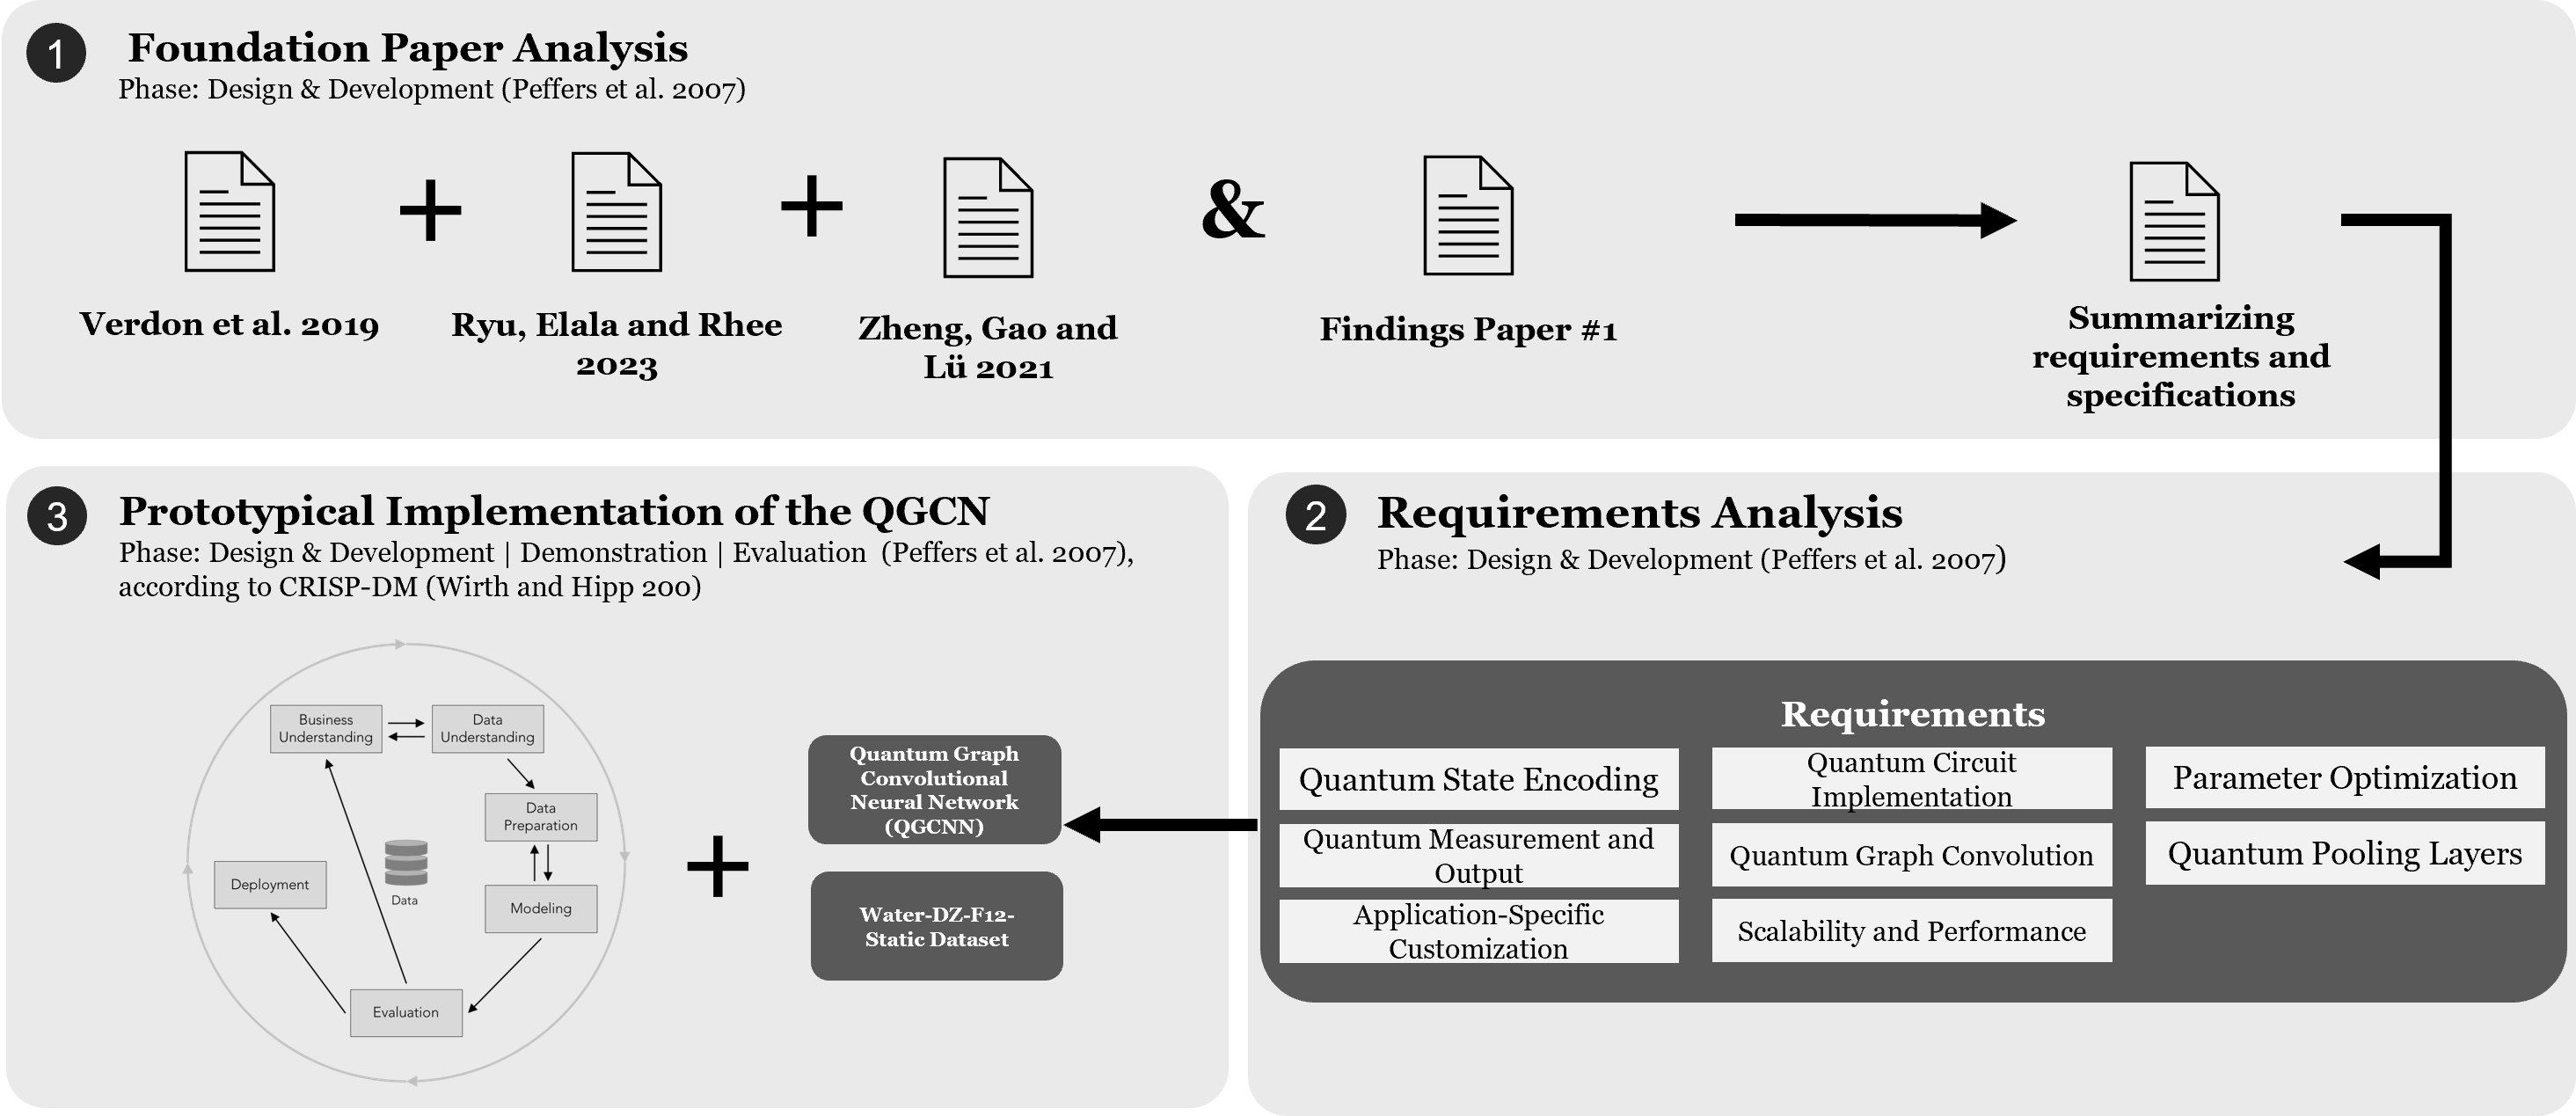
\includegraphics[width=\textwidth]{05_paper02RM.png}
    \caption[Overview of the conducted research process]{\label{img:paper02rm}{Overview of the conducted research process}}
    \end{figure} 

Three foundation papers were then analyzed to investigate different approaches to the development of QGNNs and to identify a possible approach to the development of a QGNN for the prediction of molecular properties. Similar to the results of the first paper of this thesis and the results of the foundation paper analysis, requirements for a Quantum Graph Convolutional Neural Networks (QGCN) to be developed are defined. Using these requirements, this paper will attempt to develop a prototpyical QGCN. For a better structure and traceability of the procedure, the exact research process is shown in Figure \ref{img:paper02rm} on the previous page, which is described in detail in the following section. \\

The \textbf{first step} was to analyze the foundation papers. The papers by Verdon et al. \cite{verdon_quantum_2019}, Zheng, Gao and Lü \cite{zheng2021quantum} and the paper by Ryu, Elala and Rhee \cite{ryu2023quantum} were used. Since the literature on QGNNs is limited to a very small number of papers, a structured literature analysis is not useful in this case. Accordingly, various literature databases were searched for literature on QGNNs and the papers most relevant to the topic of this thesis were selected for the foundation paper analysis. The results of the analysis of these three papers were combined with the results of the first paper of this thesis and summarized for the next step of the conducted research process. \\

In the \textbf{second step}, a requirements analysis was carried out based on the results of the foundation paper analysis. Based on the results of the first paper of this thesis, the goal was to implement a QGCN. Therefore, a total of 8 different requirements were identified for the QGCN to be developed. The results of this requirements analysis are discussed in more detail in Section \ref{subsec:requirements}. \\

The \textbf{third step} covers the prototypical implementation of the QGCN for the prediction of molecular properties. Based on the previously identified requirements, an attempt was made to implement a QGCN capable of predicting the potential energy surface using the water data set mentioned in the first paper of this thesis. Similar to the first paper, the implementation followed the structured procedure of CRISP-DM \cite{wirth2000crisp} and is explained in Section \ref{subsec:qgnndevelopment} of this thesis. Although the QGCN could not be implemented completely successfully, the development still provides interesting insights and further work can be based on the findings of this paper.

\section{Findings}
In this section, the results and findings are presented and discussed in detail. First, the analyzed foundation papers are summarized and the relevant information is extracted. Afterwards, the identified requirements given from the analysis of the foundation papers are explained in detail in the requirement analysis. As the QGCN could not be fully implemented successfully, the development of a Quantum Convolutional Neural Network (QCNN) capable of predicting potential energy surface and forming the starting point for a QGCN is demonstrated. In a final step, the challenges of implementing the QGCN are documented.

\subsection{Foundation Papers}
This section briefly summarizes all foundation papers that were read and used for the requirement analysis as shown in the first step of the conducted research process in the previous section. \\

In the paper by Verdon et al. from 2019 \cite{verdon_quantum_2019}, the authors discuss the development of Quantum Graph Neural Networks. These are quantum computing models for processing information that is represented in graph structures. The authors investigate the development of two architectures (also called ansatze in the field of quantum computing) for QGNNs: Quantum Graph Convolutional Neural Networks and Quantum Graph Recurrent Neural Networks (QGRNNs). These architectures are designed to use quantum mechanical properties to efficiently perform computational tasks on graph-structured data. Therefore, at first, the quantum circuits and algorithms on which the QGNNs ansatze are based are presented. The authors show how QGNNs can be applied to different information processing tasks, such as learning quantum hamiltonian dynamics or the execution of a graph classification task. By performing various experiments, the authors validate the proposed ansatze for the QGNNs. The performance of QGNNs in solving graph-theoretic problems is demonstrated by running simulations in comparison with classical graph neural networks. The results of these simulations show the potential of QGNNs to advance graph-based machine learning in the field of quantum computing by providing an efficient way to solve graph-theoretic problems. \\

The development and application of Quantum Graph Neural Networks for predicting the properties of molecules and materials is explored in the paper of Ryu, Elala and Rhee from 2023 \cite{ryu2023quantum}. This contribution is therefore closest to the topic of this thesis. The focus of this paper is on the prediction of the energy gap between the highest occupied and the lowest unoccupied molecular orbitals (HOMO-LUMO) of small organic molecules.  The authors present an ansatz that they call the Equivariantly Diagonalisable Unitary Quantum Graph Circuit (EDU-QGC). This ansatz is specifically designed to encode discrete bond features and optimizing the embedding process within quantum circuits, ensuring a more efficient representation of molecular structures. For the data encoding, the authors use the method of angle encoding with $R_y$ or $R_z$ gates, which is a common strategy when encoding data into the quantum state. In the EDU-QGC circuit design, the molecular bonds are represented as single or double link bonds, depending on the structure of the molecule. The authors evaluate two different readout functions: a local readout function that reads from node-local terms and a global readout functions that reads out the information given on all nodes in the graph.
In the course of experimental testing and evaluation of the developed model, the QM9-Dataset has been used by the authors, divided into 10,000 training and 1000 testing samples.  The results of the experiments conducted demonstrate the effectiveness of the QGNN model and show that it can achieve lower test losses in predicting the HOMO-LUMO gap than classical neural graph network models with a comparable number of trainable parameters. In addition, the QGNN model converges faster in the training phase, thus indicating a more efficient learning process. The authors make no general claim to the so-called "quantum advantage", but the results suggest that quantum-enhanced graph neural networks are  a promising area of research for the field of materials science and molecular chemistry. \\

The last paper describes the work of Zheng, Gao and Lü from 2021 \cite{zheng2021quantum}. In the paper, the authors describe the development of a Quantum Graph Convolutional Neural Network, which was developed for classification tasks at the graph level. They proceed according to the following steps: first, the graph data is en coded into the quantum state using amplitude encoding, next universal parameter-based gates circuits are used for the construction of the QGCN by using the amplitude encoded graph data and last, the learning ability of the QGCN is tested by training on a quantum circuit using the MNIST dataset for classification benchmarking. Accordingly, the authors develop a quantum analogue of classical graph convolutional layers that allows quantum circuits to encode graph information and perform convolutional and pooling operations. This QGCN ansatz processes graphs by encoding node features and structural information such as the connections between the nodes into quantum states, and then applying parametrized quantum gates to simulate convolutional and pooling operations. According to the authors, this ansatz makes it possible to capture patterns and relations between nodes within the graph structure. To test the proposed QGCN ansatz, the authors use the MNIST dataset in their experiments, which contains handwritten digits and is often used for benchmarking classification tasks. The results of the experiments show that the developed QGCN ansatz achieves a high accuracy of 0.90 (one convolutional layer and one pooling layer) or 0.91 (two convolutional layers and one pooling layer). These results demonstrate that graph data can be efficiently processed using quantum computing and accurate predictions can be made.

\subsection{Requirement Analysis}

Following the summary of the foundation paper, this chapter presents the requirements identified in the foundation paper. The Figure \ref{img:requirements} shows an overview of the eight requirements. These are considered and explained in detail below

\begin{figure}[h!]
    \centering
    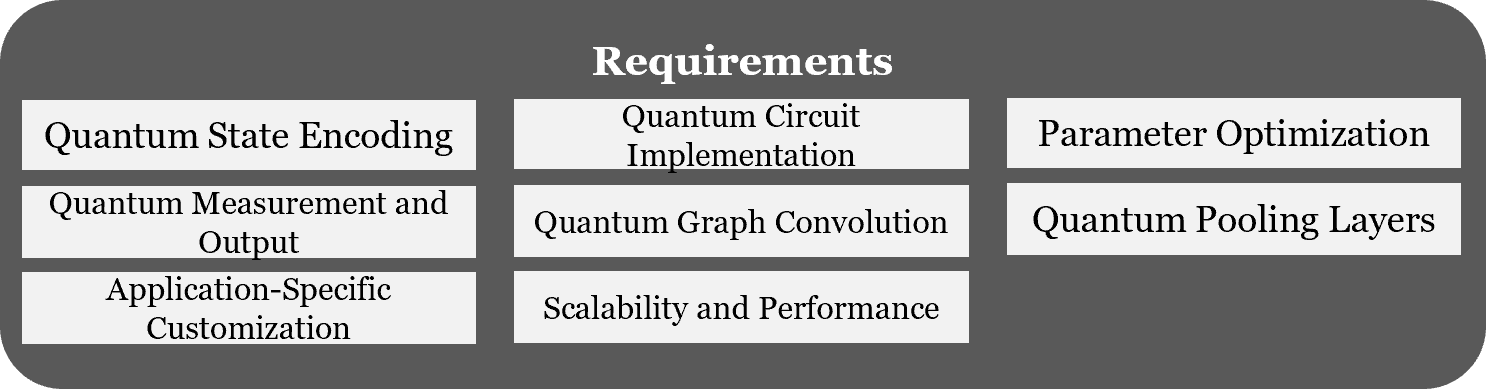
\includegraphics[width=\textwidth]{requirements.png}
    \caption[Identified requirements from the requirement analysis]{\label{img:requirements}{Identified requirements from the requirement analysis}}
    \end{figure} 

The first requirement describes quantum state coding, i.e. the encoding of classical data into quantum states. To develop a QGCN, the graph structures must be converted into quantum states. This involves encoding the node and edge information onto the qubits. Two different strategies were used in the foundation papers: amplitude encoding \cite{zheng2021quantum} and angle encoding \cite{ryu2023quantum}. The best encoding strategy depends on the underlying use case and must be tested during implementation. In the case of predicting potential energy surfaces for molecules, the atoms need to be coded with their coordinates and chemical bonds as nodes, and the regression target needs to be linked to the coordinates of the molecules. \\

The second requirement is the implementation of the quantum circuit and thus the structure of the implemented quantum circuits for data processing. Hereby, the number of qubits plays a major role. For data sets with a relatively small number of features, it is possible to map one feature onto one qubit. For graph-based data, however, it is necessary to use several qubits to map the relationships between the atoms of a molecule. In this way, the qubits are manipulated and the weights within the molecules are represented based on the atomic coordinates and chemical bonds. The design of the circuits has a major impact on the performance and accuracy of a QGCN, i.e. its ability to learn from graphically structured data and make predictions. \\

Another requirement for the QGCN to be developed is the parameter optimization. In QML or quantum circuits, parameters are used to learn and store relationships in data sets to enable later predictions. Parameter optimization is necessary to minimize the loss function when training a QGCN and to obtain accurate prediction results. This is done in a similar way to the parameters used to train classical neural networks. To learn the correlations in the data, the number of parameters should always be greater than the number of features used. \\

Quantum measurement and output comprises a further requirement resulting from the analysis of the foundation papers. This refers to the way in which measurements are performed during calculations in quantum circuits. In the field of QML, measurements are the probability distributions that result from the calculations within the quantum circuits. So-called observables are used for this purpose. The challenge is to recognize where and with how many qubits measurements should be made. For QGCNs, quantum measurement is limited to the measurement of single or double qubits after pooling operations have been carried out. In the context of QGCNs, the quantum information is translated into a form that can be used for further tasks, such as the classification of graphs. \\

The following two requirements can be summarized and describe the architecture of the QGCN in addition to data encoding and quantum measurement. These are the quantum graph convolution and quantum pooling layer requirements. Quantum graph convolution is analogous to classical convolutional operations on graph data. Parameterized quantum circuits are used to compute local and global neighborhood structures between nodes and to learn feature weights. In this way, the QGCN can recognize the connectivity and relationship patterns within a graph.

The requirement for quantum pooling layers refers to the introduction of the pooling mechanism, which is also used in classical convolutional neural networks. The pooling mechanism aims to reduce the dimensions of the feature space and thus the computational cost, while preserving the important features. In quantum pooling, the number of qubits in the QGCN is reduced by stringing together different convolutional and pooling layers to enable efficient measurement operations on one or two qubits during the training of the QGCN. \\

The application-specific adaptation of a QGCN describes the second last requirement during the development a QGCN. When designing quantum circuits, they must always be designed and implemented taking into account the underlying (graph) data and are therefore application dependent. In the case of the QGCN for predicting molecular properties, this concerns the number of qubits, the structure of the quantum circuits, the number of parameters in the quantum circuits and the number or arrangement of the convolutional and pooling layers. This ensures that the QGCN can learn effectively from the properties of the dataset and the underlying use case. This is closely related to the last requirement, scalability and performance. As quantum hardware in particular is constantly evolving, the QGCN needs to be scalable to continue to use qubits and quantum circuits to achieve improved performance and efficient use of available computational resources. This step should also ensure that data sets of different sizes can be used in the field of molecular property prediction.

\label{subsec:requirements}
\subsection{Development of the QCNN}
\label{subsec:qgnndevelopment}

After gaining insight into the requirements of a QGCN, it was attempted to develop a QGCN for the prediction of molecular properties. It was possible to develop a QCNN consisting of a convolutional layer and a pooling layer. The development of the QCNN in this paper is based on the QCNN of the Qiskit ecosystem \cite{qcnn}. However, it was not possible to fully implement the processing and interpretation of the graphs. This paper therefore documents the development of the QCNN, which can be used as the basis for a QGCN. This QCNN was trained with a data set containing only water molecules, similar to the first paper in this thesis. The development of the GCN was based on the established CRISP-DM process \cite{wirth2000crisp}, which is explained step by step below. \\

The first phase of the CRISP-DM process refers to business understanding and is essentially the same as the introduction from Chapter \ref{sec:introduction}. For reasons of focus, this phase is therefore not listed separately again. However, in the second phase of the process, data understanding, the aim is to provide an insight into the given data set. As already mentioned, a data set consisting of approx. 36,000 water molecules is used.  This data set contains molecules consisting of oxygen and hydrogen atoms, which have different atomic coordinates. The relevant target variable is also contained in the data set and describes the potential energy surface of the atom. \\

In the next step, the dataset will be prepared to be able to train the developed QCNN. The data preparation includes at first the extraction of all relevant information from the dataset, which is in this case the atoms, the cartesian coordinates of the atoms which are the features and the regression target variable. For better results off the model predictions, the target variables are normalized with the help of their mean and standard deviation. Additionally, the features are normalized between a range of 0 and 1 which is an important step before encoding data into the quantum state. \\

After the data preparation, the architecture of the QCNN is implemented during the modeling phase of the CRISP-DM process. The QCNN consist in total of nine qubits, one qubit for one feature from the input data. After the data is encoded into the quantum state, the QCNN consists of three convolutional and three pooling layers. Each pooling layer reduces the number of qubits, whereas after the last pooling layer a one qubit measurement is performed. The convolutional and pooling layers contain different amounts of parameters where the relation between the data is learned during the training. This architecture is based on the results from the requirement analysis from the previous section and can be seen in Figure \ref{img:qcnnarchitecture}. \\

\begin{figure}[h!]
    \centering
    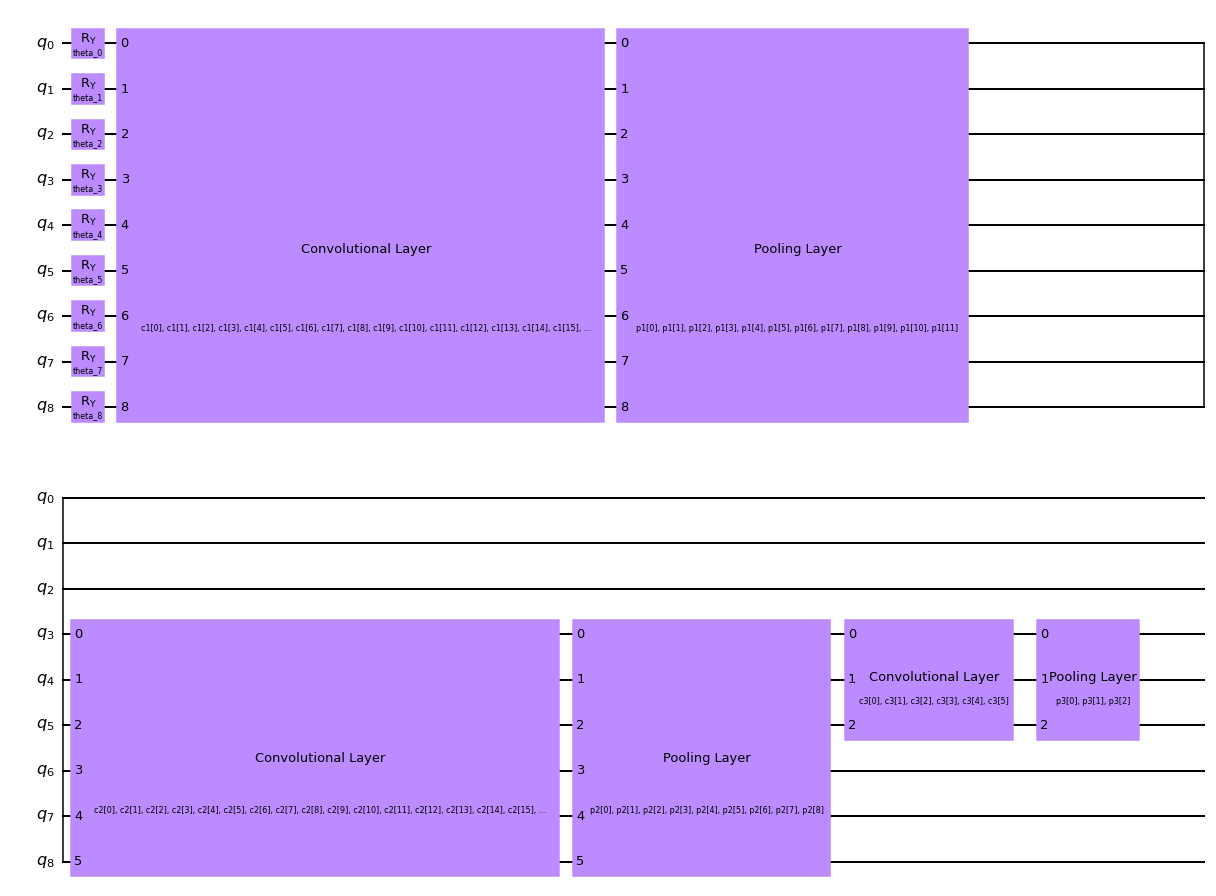
\includegraphics[width=0.65\textwidth]{qcnnarchitecture.png}
    \caption[Architecture of the developed QCNN with angle encoding]{\label{img:qcnnarchitecture}{Architecture of the developed QCNN with angle encoding}}
\end{figure} 

The second last phase describes the evaluation of the developed model, where the performance of the model is assessed. Due to concerns about the training time resulting from the simulation of quantum computations on classical hardware, the training was reduced to 40 samples from the data set. For the same reason, the results do not describe the actual calculations on a quantum computer. For comparison, the model and its performance were tested with angle and amplitude coding as suggested in the requirements analysis. During training, the model is optimized using the COBYLA optimizer algorithm, which is a common optimizer in the quantum computing context. Since the prediction of the potential energy surface is a regression task, the quantum model can be evaluated with the different regression metrics just like the classical models. The results are shown in Table \ref{tab:paper02performancecomparison}. 

\begin{table}[h!]
    \centering
    \captionsetup{justification=centering}
    \resizebox{\textwidth}{!}{
        \setlength{\tabcolsep}{1.5em}
        {\renewcommand{\arraystretch}{1.5}% for the vertical padding
            \begin{tabular}{p{7cm} l l}
                \hline
                 \textbf{Parameter} & \textbf{Amplitude Encoding} & \textbf{Angle Encoding} \\
                 \hline
                   Training time &  3 min 52.3s & 3 min 27.8s  \\
                   Mean Squared Error (MSE) & 0.2359 & 0.2150 \\
                   Root Mean Squared Error (RMSE) & 0.0667 & 0.0585 \\
                   Train data accuracy ($R^2$) &  85.87\% & 89.27\%  \\
                   Test data accuracy ($R^2$) &  85.65\% & 88.98\%  \\
                   \hline
               \end{tabular}
           }
       }
       \caption[Comparison of performance metrics of the developed model with different data encoding strategies]{\label{tab:paper02performancecomparison} Comparison of performance metrics of the developed model with different data encoding strategies}
\end{table}

As shown in the Table, training the QCNN model with similar hyperparameters ($n_{samples}$ = 40), $(n_{epochs}$ = 250) but different data encoding strategies delivers very similar results, with the angle coding giving slightly better values, for example with an accuracy of 89.27\% on the training data and 88.98\% on the test data, where the amplitude encoding only gives 85.87\% on the train data and 85.65\% on the test data. It can also be seen that the training time is about 11\% faster when using angle encoding as data encoding strategy. This gives angle coding an overall superiority over amplitude coding when it comes to predicting potential energy surfaces.\\

During the last phase of the CRISP-DM process, the developed and evaluated QCNN can be deployed and make use of the knowledge gained. In the course of this paper, the developed QCNN is a prototype and constitutes a basis for a graph-based quantum neural network model and will be used for the further developed of a graph-based model that predicts the potential energy surface of molecules. 
%\subsection{Challenges during the development}

\section{Conclusion}
Although the primary research question could only be answered theoretically, the results show a structured approach to the development of a QGCN and form a solid basis for further work. Accordingly, the research process that was carried out proved to be suitable for the answering of the underlying research questions. This chapter summarizes and critically reflects on the results and identifies future research potential.

\subsection{Summary}
During the analysis of the foundation papers, three papers were identified that provide information on the development of QGNNs. Based on these papers, a total of 8 different requirements for the implementation of a QGCN that has a similar architecture to the developed model from the first paper of this thesis could be identified. These requirements were explained individually. This approach leads to a theoretical answer to the research question of this paper. Using the information from the foundation papers and the requirements, an attempt was made to develop a QGCN that predicts the potential energy surface of molecules. As the QGCN could not be implemented completely successfully, the development was documented using a QCNN that also predicts molecular properties. Nevertheless, the research process and its results in terms of the requirements and the development of the QCNN provide valuable insights into the development of the QGCN and form a solid basis for further work. 

\subsection{Critical Reflection}
As mentioned before, the research methodology was suitable for analyzing the identified foundation papers, the extraction of the requirements and the implementation of a QCNN architecture. However, this work also has its limitations. Due to various challenges, the architecture of a graph-based quantum neural network could not be implemented. For this reason, the results of this thesis can only provide a theoretical answer to the underlying research question. This suggests that further work on the identification of requirements for QGNNs could have been investigated. However, it must be pointed out that this field of research is still very underexposed and the existing literature is thematically distant from the research question of this thesis. Therefore, it was not possible to draw a comparison between a classical and a quantum graph-based neural network, so that this research question remains unanswered. Furthermore, it should be noted that the QCNN architecture developed in this paper was only tested in simulation and no real computation was performed on quantum hardware. For this reason, no statement can be made about the quantum advantage, but the results show a promising basis for further work.

\subsection{Outlook}
The path to fully functional QGNNs for the prediction of molecular properties is still at an early stage. The results of this paper in the form of the identified requirements and the basic QCNN architecture provide a starting point for further research in this field. Due to the advances in quantum hardware and the increasing number of qubits, the development of quantum computers that are far superior to classical models will be a central aspect of future research not only for the prediction of molecular properties, but also in other research areas. The investigation of such quantum machine learning models opens up new dimensions in hydrogen research and in computational chemistry and materials science as its superordinate fields. Utilizing the power of quantum computers will make an important contribution to environmental protection and sustainability through the use of new methods and materials.